\documentclass[../report.tex]{subfiles}

\begin{document}

\begin{figure}
\centering
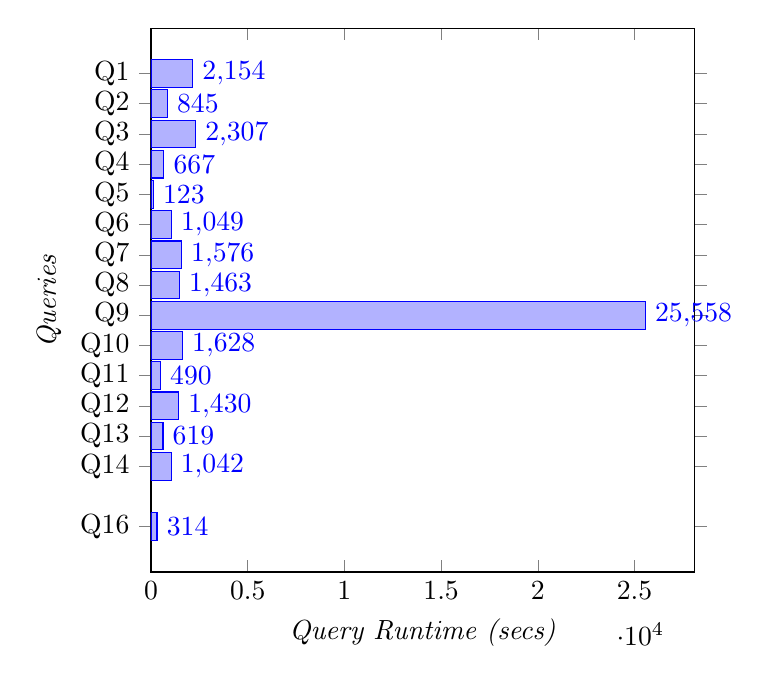
\begin{tikzpicture}[baseline]
    \begin{axis}[
            xbar,
            ytick=data,
            width=0.7\textwidth,
            height=0.7\textwidth,
            symbolic y coords={Q1,Q2,Q3,Q4,Q5,Q6,Q7,Q8,Q9,Q10,Q11,Q12,Q13,Q14,Q15,Q16,Q17,Q18,Q19,Q20,Q21,Q22},
            ylabel=\emph{Queries},
            xlabel=\emph{Query Runtime (secs)},
            % xmode=log,
            y dir=reverse,
            xmin=0,
            nodes near coords,
            nodes near coords align={horizontal},
        ]
        \addplot coordinates {
            (2154,Q1) (845,Q2) (2307,Q3) (667,Q4) (123,Q5) (1049,Q6) (1576,Q7) (1463,Q8) (25558,Q9) (1628,Q10) (490,Q11) (1430,Q12) (619,Q13) (1042,Q14) (314,Q16)
        };
    \end{axis}
\end{tikzpicture}
\label{fig:pg_time}
\caption{Queries' runtime}
\end{figure}

\end{document}
